\author{Nicolas SILVA}
\title{Un dialogue entre l'Art et l'Homme}
\documentclass[a4paper, 12pt]{article}

% Faire des marges un peu moins large que celles par défaut
\usepackage[top=20mm, bottom=20mm, left=25mm, right=25mm]{geometry}
\usepackage{ucs}
\usepackage[utf8x]{inputenc} % Pour l'encodage 
% Reconnaitre les caratères accentués dans le source.
\usepackage[T1]{fontenc} 
% Meilleurs polices
%\usepackage{concmath}
%commenter les 2 lignes suivantes pour passer en anglais
\usepackage[francais]{babel}
\NoAutoSpaceBeforeFDP

% Insertion d'images
\usepackage{graphicx}
% Pour le listing de code
%\usepackage{listings}
% Pour la coloration syntaxique
\usepackage{xcolor}
% Pour fixer l'interlignage
\usepackage{setspace} 
% Pour faire un index (ici glossaire)
\usepackage{makeidx}
% Pour gérer les liens internes et les URL cliquables
\usepackage{url}
% Pour les headers et footers
\usepackage{fancyhdr}
% Pour le logo en haut a droite
%\usepackage{eso-pic} 
% Pour l'enroulement du texte autour des figures
\usepackage{wrapfig}
% Pour la couverture en PDF pleine page
\usepackage{pdfpages} 
% Pour la biblio bibtex
\usepackage{bibunits}
% Pour gérer les éléments flottants
\usepackage{float}
% Pour les cadres à ombrage du glossaire
\usepackage{fancybox}
% Pour faire des sous-figures correctement numérotés
\usepackage{subfigure}
% Pour mettre les liens cliquables
\usepackage{hyperref}


\setlength{\headheight}{14.5pt}

\newcommand{\centeredimage}[4]{%
	\begin{center}
		\includegraphics[width=#2]{#1}
		~\\ \emph{#3},
		~\\ #4
	\end{center}
}




\usepackage{wrapfig}
\newcommand{\sideimage}[4]{%
\begin{wraptable}{r}{#2+1em}
  \begin{flushright}
  \vspace{-0.9cm}
    \includegraphics[width=#2]{#1}
  %\vspace{-0.8cm}
  ~\\ \emph{#3}, 
  ~\\#4
  \end{flushright}
  \vspace{-0.6cm}
\end{wraptable}
}


\newcommand{\xspace}{\vspace{0.6cm}}

\newcommand{\chapterseparator}{~\\ \begin{center} * * * \end{center} ~\\}

\newcommand{\partseparator}{~\\ \begin{center} * * * * * \end{center} ~\\}

% Couleur des url et des liens internes.
\hypersetup{urlcolor=blue,linkcolor=black,citecolor=black,colorlinks=true}

%headers, footers
\pagestyle{fancy}

\cfoot{\thepage}


\rhead{INSA de Lyon -- 2007/2008}
\lhead{Nicolas Silva}
\date{} 

\begin{document}
~\\
\begin{center}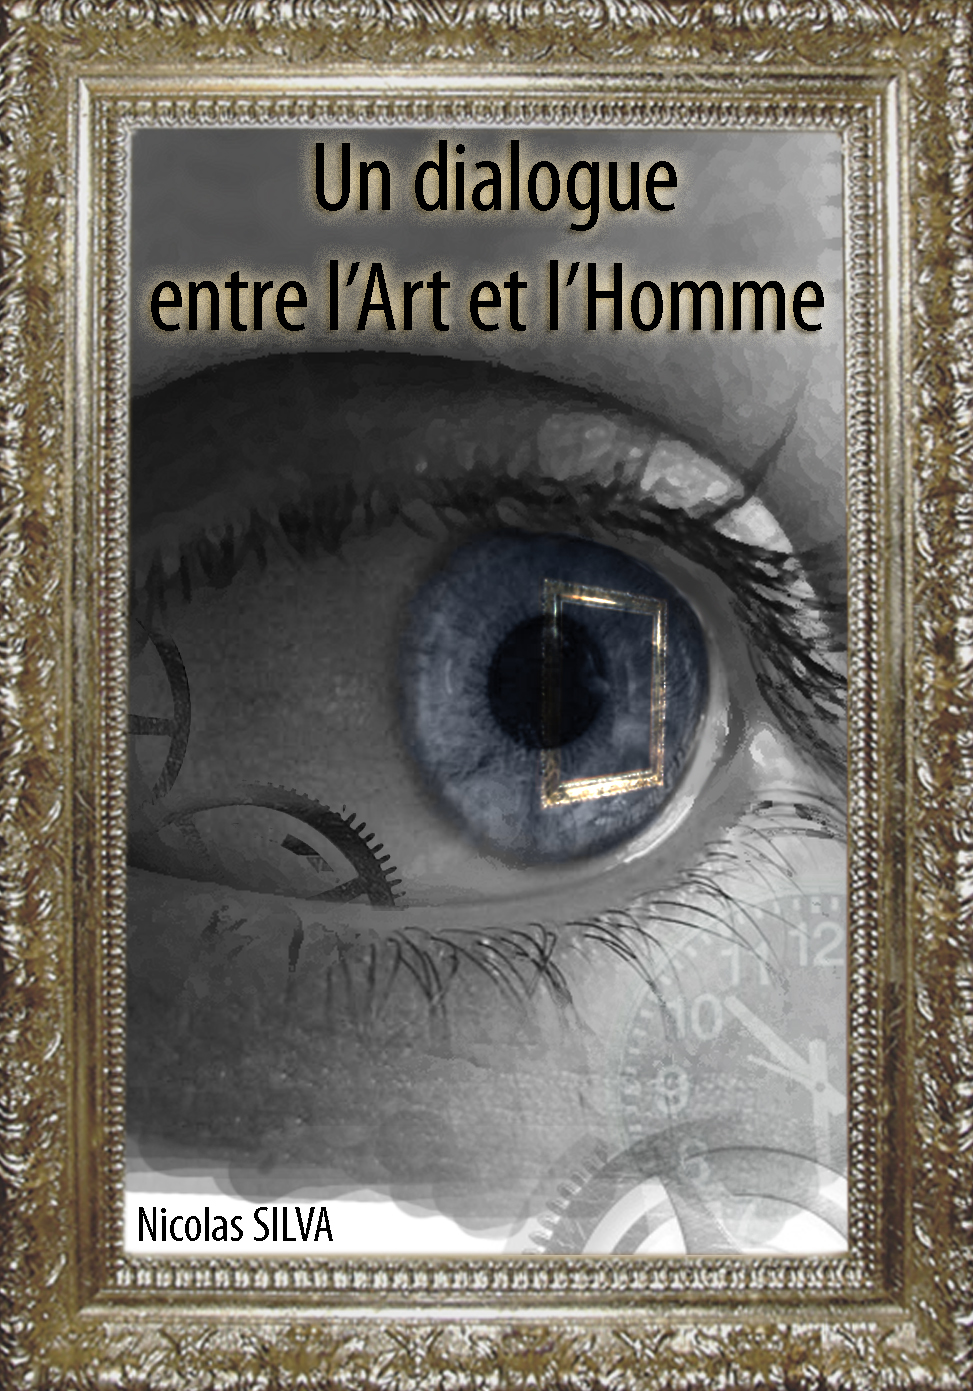
\includegraphics[width=\linewidth]{images/couverture.jpg} \end{center}
%\AddToShipoutPicture{%
%\setlength{unitlength}{1mm}%
%\put(230,420){%
%\makebox(0,0){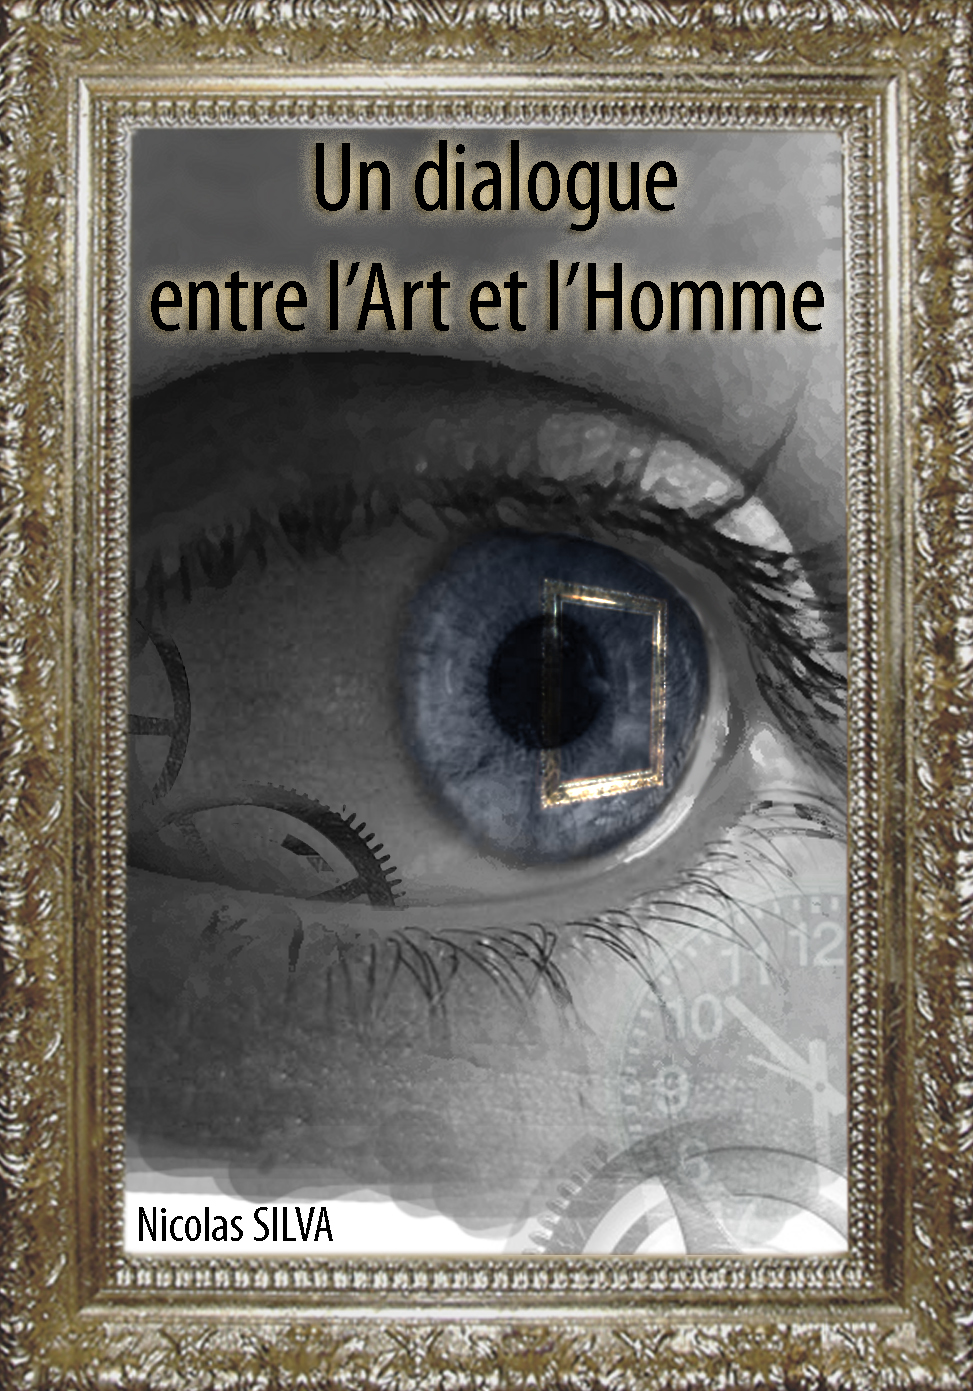
\includegraphics{images/couverture.jpg} }}}
\thispagestyle{empty}
\newpage

\maketitle
\vspace{3em}
\tableofcontents
\setcounter{page}{1}
\newpage

%-------------------------------INTRO
	 Le processus de création est un élément fondamental dans la construction psychologique et sociale de l'homme. Cette capacité de créer a permit à l'être humain non seulement de dépasser les limites que lui impose son corps, mais aussi de s'inscrire dans un processus d'évolution non plus biologique, mais historique. L'art est un des principaux signes de cette capacité d'abstraction qui confère à l'homme le pouvoir d'inventer et de créer. Nul doute que l'art est propre à l'homme, mais l'homme lui-même est-il propre à l'art ?

De quoi est fait le lien entre l'homme et l'art ? La relation entre l'art, en tant qu'objet et en tant que concept, et L'homme, en tant qu'artiste et en tant que spectateur, fera l'objet de ce dossier. Nous verrons que l'interaction n'est pas unilatérale, qu'elle n’opère pas non plus en un seul temps. En fait nous verrons que cette interaction s'apparente à un dialogue. Attention cependant : l'art est une notion extrêmement vaste, il serait trop ambitieux, voir même peu judicieux de l'étudier dans sa totalité. C'est donc au quatrième art, celui de la peinture et du dessin, aux arts plastiques que se réduira notre étude. Ajoutons même que cette étude, bien que pouvant être généralisée à de nombreuses autres cultures, s'orientera principalement vers l'art occidental, notamment en ce qui concerne les exemples qui seront traités. Ces restrictions sont nécessaires, compte tenu de l'ampleur du thème abordé, afin de rester cohérent et de pouvoir approfondir certains points intéressants.

\xspace
	La première difficulté qui se pose à l'étude de l'art est la richesse de sa dimension historique. Il n'est pas possible de mener une réflexion sur l'art sans étudier son évolution dans le temps, tant cette dernière est importante. Nous aborderons donc en premier lieu un exemple illustrant l'évolution de l'art à travers les époques. Les informations que nous tirerons de cet exemple nous seront utiles pour étudier ensuite l'évolution de l'objet d'art dans le temps et enfin l'évolution du concept artistique.

	Une fois la dimension temporelle mise en place, nous nous concentrerons sur le dialogue entre l'artiste et l'oeuvre d'art. La production artistique est un moyen d'expression et de réflexion. Nous verrons alors que la nature du lien entre créateur et création repose sur une forte volonté de transcendance, propre à l'homme, certes, mais particulièrement présente dans le processus de création.
L’artiste travaille pour un autre, un spectateur. Une fois exposée, son œuvre cesse de lui appartenir pour exister sous le regard de l’autre. Le rapport entre l’œuvre et le spectateur fondera la troisième partie de ce dossier. Nous verrons tout d’abord la puissance de l’image et du signe, puis comment l’œuvre d’art transmet, guide, et constitue un média. Enfin, nous aborderons un des points fondamentaux de l’attachement des hommes aux œuvres d’art : l’émotion qu’elles provoquent.   
	

\partseparator
\newpage
\section{Un dialogue qui évolue dans le temps}
\subsection{Evolution du support artistique : exemple par l'histoire d'une couleur}
\xspace
	L'évolution de la peinture à travers les siècles est très liée à l'histoire des couleurs. Il est important d'observer l'évolution des couleurs dans les m\oe{}urs, les techniques et l'utilisation plastique. Le pigment est le support de l'expression artistique. C'est lui que l'artiste étale sur sa toile et c'est lui que nous, spectateurs, observons. Son agencement compose l'\oe{}uvre, il véhicule le geste et l'expression de l'artiste. Or, la création de pigments n'a pas toujours été aussi maîtrisée qu'aujourd'hui. À cela ajoutons que les couleurs ont eu, au cours de leur histoire, différents statuts sociaux, et même moraux. Tout cela entraîne d'importantes répercussions sur l'histoire de l'art. L'étude des couleurs représente donc un point de départ à la compréhension de l'évolution de la peinture. Etudions de façon non exhaustive l'histoire de la couleur bleu, la couleur dont le statut a le plus évolué au cours du temps.

\xspace
	Michel Pastoureau explique dans \emph{Bleu, histoire d’une couleur} qu’on date à trois mille ans avant notre ère les plus anciennes activités de teinture sur support textile en Europe parvenues jusqu'à nous. Toutes dans des tons rouges. La primauté du rouge est encore effective dans la Rome antique, alors que la couleur bleue, elle, est presque inexistante, à tel point que certains historiens ont soutenu que les grecs et les romains ne voyaient pas cette couleur. Il est en effet difficile de traduire en grec et en latin le bleu. En grec les deux mots les plus utilisés pour désigner le bleu sont \emph{glaukos} et \emph{kyaneos}; le dernier qualifie aussi bien le bleu clair des yeux que le noir des habits de deuil, mais jamais la couleur du ciel ou de la mer. Dans la période classique il désigne un couleur sombre: bleu foncé mais aussi violet, le noir le brun. \emph{Kyaneos} traduit d'avantage le sentiment de la couleur que sa teinte. \emph{Glaucos}, terme un peu plus ancien, désigne autant le gris que le vert, parfois même des teintes brunes. Il traduit d'avantage l'idée de pâleur qu'une réelle coloration. Dans l'\emph{Iliade} et l'\emph{Odyssée} d'Homère, on note que sur soixante adjectifs qualifiants des éléments de paysages, seulement trois se rapportent à la couleur quand de nombreux autres traitent de la lumière. En latin il existe de nombreux termes (glaucus,caeruleus, caesius, cyaneus, lividus, venetus, aerius, ferreus) mais ils sont tous imprécis, polysémiques et d'emplois contradictoires. Ce n'est qu'au Moyen Âge chrétien que deux mots apparaissent dans le lexique latin: blavus, venu des langues germaniques, et azureus, venu de l'arabe. Ce sont ces deux mots qui prendront le pas sur tous les autres dans les langues romanes. Certains savants ont donc mis en avant les théories évolutionistes pour appuyer que les grecs et, à leur suite, les romains ne voyaient pas la couleur bleue. Cependant cette thèse est, comme le souligne Michel Pastoureau, trop ethnocentriste et on oublie souvent qu'il y a un écart entre la vision qui est un phénomène biologique, et la perception qui est un phénomène en grande partie culturel. Les romains n'ignorent pas la couleur bleue, ils lui sont indifférents, voire hostiles : pour eux le bleu est la couleur des Barbares, Celtes et Germains.

\xspace
	Dans les images et \oe{}uvres d'art du haut Moyen Âge, le bleu est certes discret mais joue parfois des rôles importants. Bien que n'étant qu'une couleur périphérique sans symbolique propre pendant la période paléochrétienne, il devient dans l'empire Carolingien un moyen de mettre en valeur la majesté des souverains et même quelques fois une teinte des habits de personnages divins tels que l’empereur ou la Vierge. À partir du XIe siècles, le bleu change de statut. Il n'est plus désormais une couleur de second plan, mais devient une couleur à la mode, sa place en art se fait de plus en plus importante, “la plus belle couleur” selon certains auteurs. Cette promotion de la couleur bleue se ressent particulièrement dans son statut pictural et iconographique. Dans la palette de l'artiste, le bleu sombre, assez rare chez les cultures anciennes, s'éclaircit, se fait plus séduisant.

\sideimage{images/botticelliVe.jpg}{16em}{\emph{La Vierge et l’enfant entourés de cinq anges}, Botticelli, 1470}
\xspace
	Notons que la Vierge n'a pas toujours été représentée dans une robe bleue, il faut attendre la fin du XIIe siècle pour qu'elle soit principalement associée à cette couleur. Ce changement n'est pas anodin, Marie est l'une des figures les plus importantes dans un art alors presque exclusivement religieux. Pendant cette période le bleu change de statut mais aussi de teinte, les contraintes techniques et financières concernant la production des pigments sont encore importantes. On utilise de plus en plus souvent du cuivre ou du manganèse au lieu du cobalt. Le bleu gothique de la Sainte-Chapelle vers 1250 n'a pas grand rapport avec le bleu roman de Chartres du siècle précédent.

\xspace
	Pendant la révolte protestante, ont lieu de nombreuses réformes iconoclastes, mais aussi dans un certaine mesure “chromoclastes” : on s'insurge contre les couleurs exubérantes, trop voyantes au profits d'agencements sobres. Le bleu opère comme un retour dans l'histoire : il s'assombrit et se désature. Au XVIe siècle, c'est chez Calvin que l'on trouve le plus de recommandations à propos de l'art et de la couleur. Calvin ne condamne pas les arts plastiques mais il prône que ceux-ci doivent uniquement chercher à instruire et à honorer Dieu. Non pas en représentant le créateur, ce qui est abominable, mais en représentant la création. L'artiste doit donc fuir les sujets artificiels, gratuits ou invitant à l'intrigue. L'art n'a pas de valeur en soi : il vient de Dieu et doit aider à mieux le comprendre. Pour Calvin, les éléments constructifs de la beauté sont la clarté, l'ordre et la perfection. Chez certains peintres calvinistes on observe presque un phénomène de chromophobie. Rembrandt, par exemple, s'appuyait sur des tons foncés, peu nombreux (jusqu'à parfois tendre vers la monochromie), pour laisser place à de puissants effets de lumière et de vibration. Au XVIIe siècles l'austérité chromatique se retrouve aussi chez des peintres catholiques, en particulier ceux qui s'inscrivent dans le courant janséniste. On remarque par exemple que la palette de Philippe de Champaigne devient plus sobre lorsqu'il se rapproche du jansénisme. Sa palette se rapproche de celle de Rembrandt (avec le bleu en plus) et s'éloigne de celles de peintres faisant toujours usage de couleurs saturées, comme Rubens ou Van Dyck.

\xspace
	La diversité des palettes au XVIIe siècle reflète bien le débat qui oppose depuis la Renaissance l'importance de la couleur par rapport à celle du dessin. Les adversaires de la couleur soutiennent que le dessin est plus noble que la couleur car il est une création de l'esprit et non un simple mélange de matière. 
De plus la couleur est trompeuse, séduisante, elle détourne du vrai et du bien, et ne peut être qu'artifice et fausseté Par ailleurs elle est jugée incontrôlable dans le sens où  elle se refuse au langage et échappe à l'analyse. On ne comprend alors pas encore les phénomènes physiques liés à la couleur, mais les découvertes de Newton en optique montrent entre autres que la couleur est lumière, et qu'il est possible de la mesurer. Les artistes se rangent alors de l'avis des savants au profit de la couleur. La couleur permet de guider le regard, hiérarchiser les éléments, elle montre que le dessin seul ne parvient pas à tout représenter. 

\sideimage{images/titienHommeGants.jpg}{14em}{L’homme aux gants}{Titien, 1523}

	Prenons l'exemple du rendu de la chair dans lequel certains artistes tels que Titien ont excellé à l'aide de subtiles nuances de couleur. Par dessus tout, la couleur donne vie aux êtres de chair. Par la suite, la couleur bleue ne cesse de prendre de l'ampleur, on découvre de nombreux pigments de tons et d'intensités variés, le bleu s'impose en art, mais aussi dans les textiles et les textes. Aujourd’hui le bleu est la couleur préférée, loin devant toutes les autres. 
Yves Klein privilégie longtemps le bleu outremer dans ses peintures monochromes « Je suis allé signer mon nom au dos du ciel dans un fantastique voyage... » et il ira jusqu’à déposer, en 1960, la formule de ce bleu à l’Institut National de la Propriété Industrielle. L’importance du bleu est également visible au niveau vestimentaire. Le bleu est une couleur évoquant le futur, une couleur préférentielle dans le milieu de la mode, évoquant souvent la pureté du ciel et de l'eau.

\xspace
\centeredimage{images/kleinGlobe.jpg}{7cm}{Globe terrestre bleu}{Yves Klein, 1962}



\chapterseparator
\subsection{L'objet d'Art évolue dans le temps}	
\xspace
	Cet exemple de la couleur bleue nous montre plusieurs choses. Premièrement, l'art a évolué, les \oe{}uvres produites à l'époque d'Homère son nettement différentes des oeuvres produites au XIIe siècles. L'histoire du bleu nous montre que le rapport entre l'homme et l'art du point de vue du processus créatif est très lié au contexte de l’époque, que l'art évolue. À l'époque d'Homère il n'y a pas de bleu en Art, et ce même en poésie, ou en chants; alors qu'au XIIe siècle le bleu est une couleur importante, couleur des rois et de la Vierge. Cette aspect certes très formel reflète les coutumes et l'arrière plan psychologique de l'artiste. Ainsi les m\oe{}urs changent, évoluent, et il en va donc de même pour l'objet d'art.

 	De quoi se compose un tableau? D'une somme de courbes, d'aplats : la matière picturale “agencée d'une certaine façon”. Cet agencement traduit le geste de son auteur, l'intention du peintre mais aussi un arrière plan psychologique : la vie morale, les sensations que le peintre a associé à sa création. Tout cela fait du tableau un objet complexe; complexe en soi, du point de vue de sa création, mais complexe également dans le regard qui est porté sur lui. C'est un point important car c'est celui qui transparaît le plus aujourd'hui : l'interprétation, la mise dans un contexte nouveau, l'observation à travers une culture qui a évolué. Une \oe{}uvre d'art ancienne n'est pas exactement une création artistique mais plutôt le reflet d'une création artistique. Nous contemplons un tableau de Rubens déformé par le temps, comme si une vitre s'interposait et déformait non pas l'image physique mais l'image psychologique et sensible que renvoient l'\oe{}uvre. Cette barrière nous empêche d'interroger le créateur alors on étudie les traces qu'il a laissées. Les incertitudes augmentent et les interprétations divergent. Chaque historien d'art (ces derniers étant les autorités dans le domaine) peut interpréter l'\oe{}uvre en fonction de sa sensibilité. À ce moment là comment se positionner ? L'\oe{}uvre d'art a-t-elle autant de “sens” que d'interprétations ? A-t-elle seulement un “sens” particulier ? Le contact entre l'\oe{}uvre et l'homme est d'autant plus subjectif que l'homme ne sait avec certitude que peu de chose à propos de l'\oe{}uvre qu'il contemple. Ce mystère qui plane sur l'objet d'art ancien constitue une dimension nouvelle. Une dimension portée par le temps. Face à cela on peut prendre l'\oe{}uvre pour référentiel et considérer que le spectateur a évolué ainsi que son contact avec l'\oe{}uvre. On peut tout autant prendre l'homme comme référentiel et considérer que c'est l'objet artistique qui a évolué. Dans un cas comme dans l'autre, l'homme aujourd’hui n'a pas le même rapport avec un objet d'art donné qu'un contemporain de l'auteur. Ce rapport au temps tient donc une place très importante. 

\chapterseparator
\subsection{Le concept artistique évolue dans le temps}
\xspace

	Il ne faut cependant pas s'arrêter à ce constat. Le rapport entre l'homme et l'objet d'art évolue car l'un des deux évolue, certes mais cette transformation ne concerne pas uniquement l'objet au singulier : le concept artistique se meut lui aussi. Ce qu'on entend par concept artistique est le rapport entre l'homme et l'art plutôt qu'entre l'homme et l'objet d'art.

Il semble que l'art reflète la fascination de l'homme. Jusqu'à la Renaissance, l'art est presque exclusivement religieux. L'artiste rend hommage a Dieu en représentant sa création et en représentant des scènes religieuses. Le culte et l'art sont en effet liés par la volonté de dépasser une réalité matérielle souvent pénible. Par la suite la création artistique se détache peu à peu de la tradition religieuse pour s’émerveiller de la nature non plus comme ouvrage divin mais plutôt comme univers. Les retombées de la Révolution industrielle détachent l'art du domaine du sacré pour en faire un document social et matériel. Ce que nous considérons aujourd'hui comme œuvre d'art n'a pas toujours eu ce statut.
\sideimage{images/masquewobe.jpg}{4cm}{}{Masques Wobés africains ayant inspiré Pablo Picasso}
Prenons l’exemple des masques africains devenus objets d’art dans la culture européenne après la « redécouverte » qu’en ont fait les cubistes. Ces derniers en ont alors fait la  promotion au travers de leurs propres collection. C'est en grande partie le contexte d'exposition qui transforme l'objet artistique. Au Moyen Âge un tableau était un objet de culte ou un objet décoratif, mais pas un objet à proprement parler “artistique”. Nous avons vu l'importance du contexte de création, n'oublions pas l'importance du contexte d'exposition. Si dans un premier temps on se pose la question: “pour qui était destinée cette \oe{}uvre? Dans quelles conditions d'exposition?”, on n'oublie pas pour autant que la dimension temporelle de l'objet artistique implique que l'on se demande aussi “Qui observe cette \oe{}uvre aujourd'hui, et dans quelles conditions?”. Et l'histoire apporte alors une donnée intéressante: le musée. L'idée de regrouper les \oe{}uvre, de les mettre dans un contexte non plus de décoration (ou de culte) mais dans un contexte d'exposition constitue en fait la réelle invention du concept artistique d'aujourd'hui. L'art n'est pourtant pas une invention récente, le terme vient du latin ars/artis dont le sens se rapproche plus de l’artisanat dans la conception contemporaine de l’art. Un terme ancien, donc, pour un concept qui n’est plus le même aujourd’hui. Il y a bien eu une évolution  

\chapterseparator

%----------------Transition entre les poarties 1 et 2

	L’art s’inscrit donc dans un processus historique complexe. L’exemple de la couleur bleue, qui fait figure de détail à l’échelle de toutes les facettes de la création artistique, en témoigne. Et dans cette évolution, le contact entre l’homme et l’art ne demeure pas inchangé, loin de là. Le temps séparant une œuvre et un spectateur donné est important car l’art est un phénomène culturel : la vie morale et psychologique du peintre, les sensations qu’il associe à son geste, tout comme le regard et l’interprétation du spectateur sont autant d’aspect primordiaux, puisqu’ils sont au cœur du contact entre l’homme et l’art, qui dépendent du contexte socioculturel  de création et d’exposition. Il devient donc difficile de généraliser une étude sans prendre en compte l’histoire des arts dans son intégralité. Est-il alors possible d’énoncer une définition précise et objective de l’art ?

\partseparator
\newpage

\section{Le rapport entre l'artiste et son \oe{}uvre}
\subsection{L'art comme moyen d'expression et de réflexion}
\xspace

	Nous avons vu que l'objet d'art était marqué par son contexte de création. Chaque \oe{}uvre s'inscrit dans un courant artistique qui se situe à une époque de l'Histoire de l'art. Mais l'\oe{}uvre d'art n'est pas le sujet de ce rapport au contexte, elle en est plutôt l'objet. Le sujet est en fait l'artiste, car c'est lui dont le processus créatif est guidé par les coutumes et les m\oe{}urs de son époque. Cette habitude, de confondre l'artiste et son travail est un signe évident du rapport étroit entre l'artiste et son \oe{}uvre. Chez les peintres du XVIIe, les diversités de palettes sont davantage dues à la façon de travailler et de mettre en \oe{}uvre les couleurs qu'à l'emploie de pigments différents. Elles sont aussi le reflet de sensibilités religieuses différentes: non seulement il y a une peinture catholique, protestante, mais dans chacune s'expriment des tendances ou de intensions plus nettement jésuites ou encore jansénistes.

\sideimage{images/schieleAutoportrait.jpg}{4.5cm}{Autoportrait}{Egon Schiele, 1910}

	La création plastique a une dimension personnelle intense. L'artiste se cherche, il s'étudie en même temps qu'il se perfectionne. Prenons l'exemple des très nombreux autoportraits que l'histoire de l'art nous présente. En se plaçant comme sujet, le peintre dirige son étude, son questionnement sur lui-même et l'immense diversité des autoportraits témoigne de la personnalité de chaque travail, de chaque questionnement de chaque façon d'appréhender le retour sur soi. Autoportraits de face, de dos (Lartigue), à l‘envers (Baselitz), nu (Egon Schiele ou Suzanne Valadon), doubles ou dans un miroir (Dubuffet), déguisé (Malévitch comme Van Dongen), avec un masque (Popovic), la diversité n'est pas uniquement portée par le choix de la pose ou la mise en situation. Baselitz, Buffet, César, Degas, Derain, Dubuffet, Max Ernst, Giacometti, Frida Kahlo, Fernand Léger, Malevitch, Matisse, Miró, Mondrian, Picabia, Picasso, Vasarely, Vlaminck, Vuillard, pour ne citer que des artistes exposés en 2004 au musée du Luxembourg à l'occasion de l'exposition "MOI ! - Autoportraits du XXème siècle –", présentent une extraordinaire diversité dans un domaine si précis, et ce au cours d'un seul siècle ! L'étude de ces autoportraits dépasserait largement le cadre de ce dossier, aussi contentons-nous de voir à quel point la peinture permet à l'artiste de s'explorer, de se faire sujet de sa réflexion. Cette réflexion ne s'arrête pas au niveau personnel. Par exemple, les vanités que nous évoquerons par la suite sont des réflexions sur la condition humaine, plus précisément sur la vanité de la vie face au statut de mortel.


%\sideimageleft{images/malevitchAutoportrait.jpg}{4cm}{Autoportrait}{Casimir Malévitch, 1933}

\chapterseparator
\newpage
\subsection{L'Art comme création, la recherche de transcendance} 
\xspace

\sideimage{images/vasarely-feny.jpg}{5cm}{Feny}{Victor Vasarely, 1963}
	L’art est un moyen pour l'homme d'évoluer dans la quête de transcendance. Chacun cherche à se dépasser dans un domaine. Le sportif, par exemple, sonde les limites de son corps quand le scientifique et le philosophe cherchent à approfondir un savoir et une compréhension de l'univers. De même, l'homme croyant en Dieu cherche des réponses aux questions que pose son existence et un moyen d'échapper à la mort. Chaque fois il est question de se dépasser, d'évoluer. L'artiste recherche lui aussi plusieurs formes de transcendances, à travers la technique par exemple. Victor Vasarely a passé sa vie à travailler une technique de dessin pour arriver à des rendus vertigineux proche de la perfection au sens géométrique.
\sideimage{images/casoEscaping.jpg}{7cm}{Escaping critcism}{Caso, huile sur toile, 1874}
L'unité entre l'art et le beau a été une évidence pendant longtemps. L'art classique était poussé par la recherche de l'esthétique, la recherche d'une beauté qui rend hommage à Dieu et à la nature. Le réalisme fût au centre de la recherche artistique depuis le Moyen Âge, surtout au XVIIe siècles, jusqu'au XXe siècle. De nombreux trompe-l'oeil sont produits au cours de cette période. Au Moyen Âge c'est donc en grande partie dans la technicité du peintre que se concentre l'activité artistique. L'artiste recherche une forme de perfection.

\xspace
	Pourquoi cette recherche de réalisme a-t-elle cessé de stimuler le milieu artistique? Plusieurs facteurs semblent entrer en jeu. Dans un premier temps l'Homme a cessé de combattre la nature pour survivre pour arriver à la dominer. Les progrès scientifiques ont amoindri la fascination que l'homme éprouvait à l'égard de la nature. En adjoignant le recul de la religion fasse à l'athéisme plus matérialiste, on arrive à une conception différente de la vision antique de la nature. Elle n'est plus la formidable création de Dieu, mais plutôt le terrain de l'homme. C'est “la mort de Dieu” dont parle Nietzsche. Le Réalisme, mouvement artistique du XIXe siècle, se place au centre du tournant qu'a pris la perception de la nature par l'homme, et plus précisément par l'artiste. Alors que le Néoclassicisme se réfère à la pensée antique d'un idéal parfait, mesuré et équilibré,  le réalisme veut montrer ce qu'il perçoit de manière objective.  Cette pensée est liée aux avancées techniques qui ont lieu à cette époque, notamment la Révolution industrielle, mais aussi du recul de la religion. la 
science prend la place des mythes. Appliquant une méthode dérivée de la méthode scientifique, l'artiste représente ce qu'il voit et non plus des scènes importantes ou des sujets mythologiques. Les paysans ou les gens du peuple deviennent des sujets de tableaux. Par la suite recherche du rendu réaliste est mise à l'écart au profit de rendus plus graphiques avec l'arrivée de l'Impressionnisme, puis du Pointillisme et du Fauvisme.

\sideimage{images/vlaminckBateaux.jpg}{7cm}{Les bateaux-lavoirs}{Maurice Vlaminck, 1906 (le Fauvisme)}
	Par ailleurs, la recherche d'une esthétique réaliste s'inscrit dans des courants artistiques, et l'Histoire des arts nous montre que  passé un temps, le processus de création nécessite du renouveau. Cette dynamique qui maintient la créativité entraîne en contrepartie la mise à l'écart de la plupart des principes de représentation qui ont déjà été exploré. Notons que  notre époque est marquée par une constante recherche de la perfection physique, et ce non plus au niveau artistique, mais au niveau social, vestimentaire et commercial. Nous sommes constamment confrontés à notre image car notre reflet est partout, le miroir n'a pas toujours existé, cela implique une certaine banalisation de la recherche esthétique : l'art ne peut plus se contenter de chercher le beau et le réaliste une fois que la technique a banalisé ce type de rendu et que les domaines du média et de la vente s'en sont emparés. Bien qu'aujourd'hui la rupture soit nette entre l'artiste et l'illustrateur, le moyen Âge ne connaissait pas de différence entre deux types de créations visuelles : l'artiste est l'artisan, art et technique étaient alors étroitement liés.

\xspace
\sideimage{images/ambassadeurs.jpg}{7cm}{Les ambassadeurs}{Hans Holbein le Jeune, 1533. ~\\ National Gallery (Londres)}
	Ce dépassement de soi n'est pas uniquement un dépassement technique, l'artiste veut surpasser son geste, sa créativité, mais aussi sa condition : l'artiste est mortel, sa vie est limitée par le temps alors que son \oe{}uvre, elle, a la possibilité de durer bien plus. L'\oe{}uvre d'art représente donc une occasion de laisser une trace intemporelle de soi, même après la mort. Tous les grands peintres se sont plusieurs fois représentés, dans des autoportraits mais aussi dans d'autres types d'\oe{}uvre dont ils ne sont pas l'objet, comme Albreitch Durër dans \emph{a fête aux couronnes de rose}. Un symbole est récurrent dans ces \oe{}uvre : le crâne qui fait directement référence à la mort. On appelle ces tableaux des vanités. Il est important de bien comprendre cet effet majeur de la capacité d’abstraction de l’homme : l’être humain peut concevoir, c'est-à-dire élaborer des objets mentaux et techniques, et cette capacité le met en face d’une force qui le dépasse et l’effraie : l’homme meurt, et il conçoit l’idée de mort. Cette idée est effrayante, à tel point qu’elle est, selon de nombreux philosophes tels que Blaise Pascal, à la base du comportement individuel et surtout social. Cependant, cette même capacité d’abstraction qui place l’homme devant la peur de mourir lui donne par ailleurs le pouvoir de se dépasser en créant. La notion de création est certainement très délicate car elle nous est naturelle et est souvent confondue avec la notion de production, cependant il est essentiel de garder à l’esprit que créer s’accompagne systématiquement d’une forme interaction avec le monde extérieur, qui est à l’échelle humaine un élément intemporel.


	
	Le rapport entre l’artiste et son œuvre est donc guidé par le processus psychologique sous-jacent à la création : la recherche de transcendance. La peur de la mort pousse l’homme à trouver des moyens de dépasser sa condition corporelle et mortelle : l’homme, et en particulier l’artiste, repousse les limites de son corps et invente l’Histoire. De plus toute l’abstraction mise en œuvre dans le processus artistique entraîne une forme de réflexion, souvent transmis intentionnellement par l’artiste. Une autre forme de dépassement se situe dans la capacité à transmettre par le biais d’un moyen original : l’œuvre d’art, qui se munit d’un langage visuel comme nous allons le voir par la suite. L’art est donc aussi un moyen d’expression et de réflexion, l’art possède une dimension médiatique. Ainsi l'artiste crée-t-il pour lui même ou crée-t-il pour ceux qui regarderont son œuvre ?  


\partseparator
\newpage

\section{Le rapport entre l'\oe{}uvre et le spectateur}
\subsection{La puissance de l'image et du signe}
\xspace

	L'impact des arts plastiques sur l'homme tient en grande partie à l'efficacité de l'image, et plus précisément du signe. Le signe est la figuration, la représentation d'un objet, d'un être ou d'un concept. Par analogie au langage écrit, le signe est en un sens l'alphabet du langage visuel. “Le signe fait balle sur la rétine. À coup sûr cette carcasse fracassée et incendiée d'automobile qu'aux Etats Unis on a parfois eu l'idée de hisser sur un socle de ciment au bord des routes ou les excès de vitesses sont courants, entraîne la pression du pied sur le frein bien plus sûrement qu'un long discours.” explique René Huyghe dans \emph{Dialogue avec le visible}. Le visuel touche directement le sens le plus important dans la perception de l'environnement, on a naturellement tendance à assimiler ce que l'on voit et ce qui est. Cette force de la figuration visuel semble même tendre à remplacer le langage écrit. Il est certes un peu tôt pour que l'historien en fasse un état de fait, mais on peu constater que les mots de la civilisation du livre reculent devant l'image qui prend de l'ampleur. La phrase au XVIIe siècle est longue, a des périodes, c'est l'époque de la dissertation où la pensée vise à s'amplifier par la forme qui l'exprime jusqu'à atteindre souvent une certaine redondance. Aujourd'hui c'est l'image qui est devenu le premier média, le média pour divertir, pour convaincre, pour vendre. L'image et même son successeur : la vidéo qui permet de mettre l'image en mouvement et de l'accompagner de sons, afin de lui donner toujours plus de crédibilité et d'impact sur le spectateur. L'Art n'a d'ailleurs pas manqué cette évolution technique. Des artistes tels que Nam Jun Paik ont exploité le support vidéo dès ses balbutiements. L'\oe{}uvre de Keith Haring, sur laquelle nous reviendrons, constitue un autre exemple de l'utilisation et de la force du signe et du symbole. De même que la numération arabe, bien plus maniable que la numération romaine, a permis aux mathématiques un bond en avant, la figuration visuelle de notions qui auparavant se développaient dans la pensée a allégé la démarche de l'esprit. Descartes rendait l'algèbre visible et l'inscrivait dans l'espace des graphiques. Leur avantage est de “parler aux yeux”. Descartes lui-même soutenait qu'avec leur aide on pouvait construire tous les problèmes, c'est à dire leur donner une forme, les transformer en image. Il découvrait que l'on peut percevoir plus rapidement, plus globalement et plus précisément avec des images qu'avec des idées. Ainsi, les fonctions et leurs courbes représentatives permettent de visualiser d'emblée des connaissances mathématiques et physiques sans se perdre dans l'énoncé du discours mental souvent bien plus compliqué. 

\xspace
	Notons cependant que cette efficacité de l'image sur l'esprit entraîne dans bien des cas un recul de la logique rationnelle au profit d'une "logique visuelle" factice. La remise en question de ce qui nous est présenté graphiquement, ou plus généralement visuellement, n'est pas spontanée et bien souvent négligée. Un graphique présentant une évolution donnée peut pour des raisons physiques admises avoir à se stabiliser à un certain moment, le plus souvent une croissance ne peut aller au delà d'un certain seuil. La montée du graphique suggère une diagonale dont l'oeil attend une continuité régulière. Une fois le seuil atteint  une horizontale prend brusquement la suite de la diagonale et, bien que ce changement soit attendu par l'esprit, pour le regard il introduit une cassure, une anomalie. En se servant de tels effets on peut susciter des sensations: une impression, une inquiétude, une panique pourtant dépourvues de fondement. Ce procédé est, par exemple, utilisé dans plusieurs œuvres présentés dans le cadre de l’exposition sur la figuration narrative qui a lieu actuellement au Grand Palais : dans l’œuvre d’Adami ci après, l’observateur est déstabilisé par des proportions, des entassements inhabituels qui renforcent son inquiétude et la violence qu’exprime l’artiste. 

\xspace
	L'efficacité du visuel et du signe est aussi liée aux courts-circuits qu'ils ont permis dans le processus de raisonnement. En remplaçant des expériences sensibles particulières par des abstractions généralisées on a permis à l'intelligence humaine de dépasser ses limites: en remplaçant des notions de pensées par des signes on arrive, par exemple à concevoir la notion d'infini qui fait buter l'esprit. On ne sait  concevoir l'infini que par une succession d'additions poursuivie sans fin, mais en y plaçant un symbole conventionnel on se dispense d'une équivalence mentale impossible pour l'utiliser empiriquement. Le signe peut donc aller plus loin que la pensée, ou plutôt permettre à cette dernière de se dépasser en faisant usage de sa capacité d'abstraction. Le Fauvisme et plus encore l'Expressionnisme ont découvert le retentissement psychique de l'image. Lignes et couleurs ont un pouvoir d'évocation qui de la sensation amène à l'émotion. Le Surréalisme est allé plus loin : l'image n'agit  pas seulement sur la pensée mais aussi sur le subconscient.

\chapterseparator
\subsection{L'Art comme média}
\xspace

	Nous avons évoqué précédemment l'efficacité de l'image en tant que média. Bien qu'il soit important de ne pas confondre les arts plastiques avec les domaines de la publicité et de l'information, ces univers ne sont pas pour autant tout à fait hermétiques.\sideimage{images/haringUntitled.jpg}{5cm}{Untitled}{Keith Haring, 1983} Prenons comme exemple l'\oe{}uvre de Keith Haring, certainement l'artiste l’un des artistes les plus importants du Pop Art après Andy Warhol.  L'artiste new-yorkais, né en 1958 et mort du sida à l'age de 31 ans, connaît très vite un grand succès. Très influencé par les univers enfantins de dessins animés, le travail de Keith Haring relie en permanence le milieu des arts plastiques au monde de la rue et de la consommation, touchant un public très large diversifié. Il développe une symbolique colorée, liée au monde des médias et se distingue en créant une iconographie unique, aux formes synthétisées. Sa technique se fonde sur un procédé rapide, il passe rarement plus de deux heures sur une \oe{}uvre, ce qui lui permet une production impressionnante en un sens comparable à la production industrielle. Sa volonté de créer un art populaire toujours plus proche du monde de la consommation se traduit par une prédilection pour des supports hors normes accessibles à tous : le métro, les murs de la ville, les réverbères, jusqu'aux produits dérivés qu'il commercialise lui-même. 
L'étonnant Pop Shop Tokyo (1985) illustre sa volonté de mettre l'art à la portée de tous et nous plonge du sol au plafond dans une vraie boutique qui permettait de diffuser son \oe{}uvre directement au grand public. Au delà de sa technique, qui lui donne ce pouvoir de diffusion, Keith Haring est aussi un artiste très engagé, dont l'\oe{}uvre présente une lutte contre la violence et le racisme. L'\oe{}uvre de cet artiste des années 80 montre bien que les arts plastiques possèdent un pouvoir de diffusion. Keith Haring est loin d'être le seul exemple possible, en réalité 

c'est l'ensemble du Pop art que l'on pourrait étudier sans même être exhaustif. L'art a non seulement la possibilité de diffuser un message, aussi une grande efficacité dans la transmission du message, comme nous l'avons vu avec l'impact du signe et comme le montre le succès fulgurant de l'\oe{}uvre de Keith Haring.
L'art contemporain semble suivre une volonté de transmettre, de toucher, voire dans bien des cas de choquer le spectateur. Le processus vise donc à faire réfléchir le spectateur, cela constitue un nouvel élément dans ce que transmettent les Arts plastiques à l'Homme.
Cette utilisation de la peinture comme moyen transmettre n'en est pas pour autant récente. Nombre d'\oe{}uvres du Moyen Âge occidental des objets de cultes visaient à guider les croyants. Parmi celles-ci on citera le Retable du jugement dernier de Rogier van der Weyden. Ce triptyque monumental est exposé à l'hôpital de Beaune, dans un dortoir où sommeillaient, au temps de sa création, les malades et les blessés. Placé à une extrémité de cet espace, derrière l'autel de telle sorte que les patients pouvaient admirer l'\oe{}uvre depuis leurs lits. Sur la surface intérieure du retable est représentée la scène du jugement dernier rappelant aux malades à la fois leur fin mortelle et leur devoir de tourner leur esprit vers Dieu. Le retable rappelait également que le soin spirituel est aussi important que celui du corps.
\xspace
\centeredimage{images/retableJugement.jpg}{10cm}{Retable du jugement dernier(ouvert)}{Rogier Van der Weyden), vers 1447} \xspace
Par ailleurs la peinture est un moyen efficace de conter : tant d'\oe{}uvres nous racontent les grands passages des différentes mythologies en utilisant une foule de détails qui, dans la scène représentée, acquièrent une protée narrative. C'est le cas par exemple de Mars et Vénus surpris par Vulcain, peint par le Tintoret en 1551 (cf. annexe : fiche de lecture). Les Arts plastiques ont donc bien un pouvoir médiatique au sens où ils peuvent, avec l'efficacité que leur confère leur forme visuelle, transmettre un message, raconter, militer, guider le spectateur ou simplement le pousser à réfléchir.


\chapterseparator
\subsection{La recherche de l'émotion}
\xspace

	Cette volonté caractéristique de l'art contemporain de créer un impact fort chez le spectateur semble mettre les plasticiens d'aujourd'hui dans une tout autre catégorie que ceux d'hier. Il est vrai que l'art d'aujourd’hui déroute, et même bien trop souvent dégoûte. On ne compte plus les artistes qui produisent des \oe{}uvres se fondant sur une forme de laideur. 
La Fontaine de Duchamp, par exemple, a fait l'effet d'une bombe détruisant l'idée que l'art était le reflet du beau. Cette \oe{}uvre, bien qu'étant en quelque sorte l'emblème, le stéréotype de l'art contemporain, n'a pas tout de suite été considérée comme objet d'art. L'urinoir constituait initialement une blague pour épater le New York mondain du salon des Arensberg que fréquentait alors l'artiste. L'\oe{}uvre a d'abord été décrétée “non artistique“ par la Society of Independent Artists.

\sideimage{images/duchamp.jpg}{5cm}{Fontaine}{vMarcel Duchamp, 1917}
Ce n'est que bien plus tard, dans le cadre de la première grande rétrospective dadaïste, au Pasadena Museum of Art de Los Angeles, qu'il est demandé à Marcel Duchamp de récréer la Fontaine. Par son succès l’objet obtient un statut d'\oe{}uvre d'art et Duchamp reçoit pas moins de vingt demandes de nouvelles fontaines. Que retient-on de cette anecdote ? Dans un premier temps, que c'est principalement ce très bref passage de l'histoire de l'art qui a marqué un tournant extrêmement important : l'\oe{}uvre d'art prend une complète indépendance vis à vis de la dimension artisanale. Artisanat qui était, rappelons le, le sens  premier du mot “art” au Moyen Âge. La Fontaine fait en effet partie des “ready made” de l'artiste, nom tout à fait explicite désignant ses \oe{}uvres qu'il n'a pas créé lui même. Retenons par ailleurs le détail suivant : l'\oe{}uvre au départ n'en était pas réellement une, mais plutôt une farce de l'artiste. Etonnant, pour un objet qui est aujourd’hui l'emblème de tout un courant artistique. Il semble que cette \oe{}uvre ait su susciter chez le spectateur, chez le critique d'art et même dans tout le milieu artistique, une émotion ou une réflexion à telle enseigne que les artistes de la figuration narrative ont éprouvé le besoin d’ « assassiner » Marcel Duchamp dans une suite de tableaux qui font référence à son urinoir. 

\centeredimage{images/finMarcel.jpg}{10cm}{Vivre et laisser mourir ou la fin tragique de Marcel Duchamp}{Gilles Aillaud, Eduardo Arroyo et Antonio Recalcati, 1965. }

 Qu'est-ce qui fait le succès de cet urinoir renversé ? \emph{La Fontaine} de Duchamp a en fait renversé les dogmes artistiques. La polémique engendrée par cette invention à entraîné bien des réflexions, et c'est sur ce point précis que l'on peut la rattacher au reste des créations plastiques : l'art de notre temps cherche l'émotion et la réflexion. Ainsi, alors qu'on a longtemps cherché à émouvoir par le beau, c'est aujourd'hui une esthétique bien plus conceptuelle qui est visée. L'art contemporain invente peu dans le domaine de la technique, l'artiste cherche maintenant à inventer dans le concept. Il doit se démarquer, il s'agit d'une course à l'invention qui repose non plus sur un talent technique, mais plutôt sur la recherche d'une idée que personne n'a eue auparavant. Ce caractère novateur entraîne alors tantôt réflexion, tantôt émotion, quoi qu'il en soit le spectateur est interpellé. Et cet accent sur l’esthétique est important car c’est lui qui élargit le public de l’art. En effet l’esthétique touche facilement le spectateur quel que soit son niveau d’éducation, puisqu’elle agit directement au niveau sensoriel sans passer par un langage ou un code particulier.

\xspace
	Remontons le temps. Quelques siècles suffisent pour se rendre compte que cette implication du spectateur n'est pas nouvelle. L'art avant Duchamp cherchait le beau afin d'émouvoir l'homme qui le regarde. Il y a toujours eu en art la recherche d'une esthétique. Bien qu'aujourd’hui il s'agit d'une esthétique du concept, l'artiste a d'abord cherché la beauté dans le monde : la beauté dans Dieu, dans la nature et dans l'homme et son action. S'il y a une beauté dans l'objet d'art, cette beauté n'a de sens que dans l'oeil du spectateur. Ceci est important du point de vue de l'effet de l'art sur le spectateur, mais aussi dans l'autre sens : l'homme est parfois sujet de l'\oe{}uvre, mais il est toujours sujet de l'intention du peintre. L'art s'adresse à l'homme et dépend de l'homme. L'art est un phénomène culturel dans le sen où il est lié à la vie de son artiste, mais aussi parce qu’il est lié à celle de ses spectateurs. En effet une \oe{}uvre d'art est avant tout un objet perçu. Nous avons vu par exemple que le musée représentait une caractéristique majeure du concept artistique d'aujourd'hui, et il en est ainsi parce qu'il a un impact direct sur le mode et le contexte de perception. Le spectateur est le censeur, le sujet final en un sens, et cela fait de lui le juge. Ce terme semble convenir au rôle de l'homme face à l'\oe{}uvre d'art et l'anecdote de la Fontaine de Duchamp en témoigne, tout comme les histoires de ces nombreux artistes qui ne furent reconnus qu'après leur mort. Aujourd'hui, comme à toute les époques, l'objet d'art est soumis au jugement de ceux qui l'observent. 

\xspace
	Daniel Arasse, \emph{dans On n’y voit rien : descriptions}, propose une réflexion sur la façon d'observer, d'analyser et de s'ouvrir aux \oe{}uvres des grands peintres en opposant deux approches différentes. La première, très savante, se base sur une lecture iconographique de l’œuvre tandis que la seconde, celle que défend Arasse, est plus sensualiste : selon lui les écrits et autres références ne doivent intervenir qu'après une observation sensible d'un tableau, sans quoi ils risquent de faire obstacle à la compréhension. Ainsi l’\oe{}uvre d'art est plus qu'un langage symbolique et la connaissance de l’iconographie et de l’histoire de l’art sont certes des outils, mais doivent seconder une exploration sensible de l'\oe{}uvre.


\partseparator
\newpage
\section*{Conclusion}
	Le dialogue  entre l’homme et l’art est riche et complexe. Les fruits de ce dialogue sont l’émotion, l’interpellation, le questionnement. L’œuvre d’art fait appel à notre capacité d’abstraction mais aussi à notre psychologie. Elle est là pour nous interpeller ainsi que pour transmettre, qu’il s’agisse du message de l’artiste ou d’une vision sociale à un moment donné. L’œuvre d’art nous incite à observer un ailleurs, à déchiffrer des signes. C’est un média utilisé par l’artiste et ses commanditaires : église, puissance publique pour transmettre des visions, des messages.
L’œuvre d’art nous provoque et elle nous construit. Nous la regardons et nous la déformons, voyant en elle ce que nous voulons ou pouvons y voir dans notre propre contexte et avec le regard de notre époque.  En ce sens le dialogue entre l’homme et l’art évolue dans le temps. L’œuvre d’art nous questionne  sur cet ailleurs qu’elle représente et sur cet autre qu’elle portraitise. Elle nous interroge également sur cet autre qu’est  l’artiste, qui l’a produit. 
L’artiste met toute son énergie pour susciter l’émotion. Pour créer, il se dépasse et  cette transcendance devient sa raison d’être. L’artiste crée pour les autres, pour exprimer, protester, transmettre, donner du plaisir,  mais il crée aussi pour lui même : dépasser la frontière de la mort en laissant une œuvre et un nom. 
Ce qui a été voulu par l’artiste n’est pas toujours ce que nous percevons et à un moment donné. Des années, des siècles plus tard ou des kilomètres plus loin, ce qui relie l’artiste au à l’homme qui regarde son œuvre c’est l‘émotion. L’émotion est l’objet central et permanent de l’art et tout ce qui est mis en œuvre dans la création artistique est investi pour susciter l’émotion ; émotion intellectuelle ou sensuelle. C’est par elle que nous allons « rentrer dans l’œuvre » et cheminer. 

\partseparator
\newpage
\section{Bibliographie}
\vspace{5em}

Livres :
\begin{itemize}
	\item \emph{On n’y voit rien : descriptions}, Daniel Arasse, 2003.
	\item \emph{Dialogue avec le visible}, René Huyges, 1955.
	\item \emph{Bleu, histoire d’une couleur}, Michel Pastoureau, 2000.
	\item \emph{Le petit livre des couleurs}, Michel Pastoureau et Dominique Simonnet, 2004.
\end{itemize}

\vspace{3em}

Sites internet :
\begin{itemize}
	\item \url{http://www.senat.fr/evenement/moi/index.html} (Exposition "MOI ! - Autoportraits du XXème siècle –").
	\item \url{www.wikipedia.org} (Biographie de Marcel Duchamp ainsi que de nombreuses images du dossier).
\end{itemize}

\vspace{3em}

Exposition :
Keith Haring, musée d’art contemporain de lyon, 2008.

\vspace{2cm}
\chapterseparator
\end{document}
